\subsection{Typedefs}
\begin{multicols}{2}
\begin{figure}[H]
    \centering
    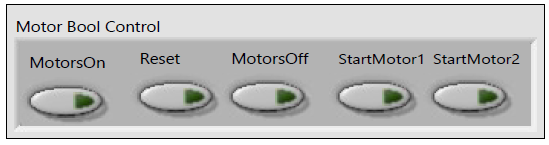
\includegraphics[width=0.5\linewidth]{vis/Motor Bool control.PNG}
    \caption{\Gls{type} av de \glspl{boolean} sendt over Modbus-tilkoblingen.}
    \label{fig:MotorBoolCl}
\end{figure}
\begin{figure}[H]
    \centering
    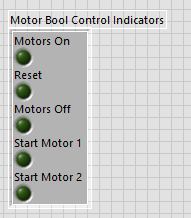
\includegraphics[width=0.5\linewidth]{vis/Motor Bool Indicatorsl.PNG}
    \caption{\Gls{type} av de \glspl{boolean} mottatt over Modbus-tilkoblingen.}
    \label{fig:MotorBoolInd}
\end{figure}
\begin{figure}[H]
    \centering
    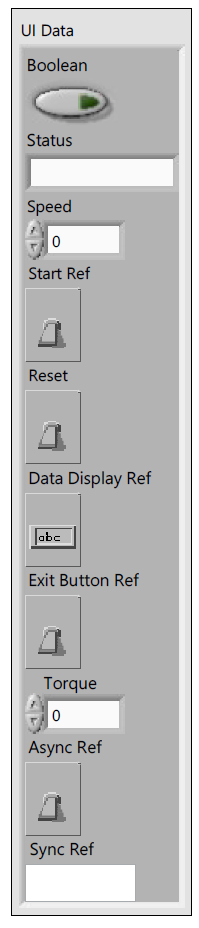
\includegraphics[scale=0.5]{vis/UI.PNG}
    \caption{\Gls{type} av elementene i \glset{bg}.}
    \label{fig:UI}
\end{figure}
\end{multicols}
\subsection{Helper VIs}
\begin{figure}[H]
    \centering
    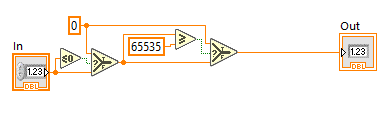
\includegraphics[width=0.5\linewidth]{vis/Remove invalid values.PNG}
    \caption{\textit{RemoveInvalidValues.vi} er en hjelpe \Gls{vi} som fjerner ugyldige verdier. Fordi en 16-bit \gls{word}, uten fortegn som blir send over Modbus-tilkoblingen kun kan ha heltallsverdier mellom $0$ og $2^{16} = 65535$. Any value outside this range is forced to be either $0$ or $65535$.}
    \label{fig:RIV}
\end{figure}
\begin{figure}[H]
    \centering
    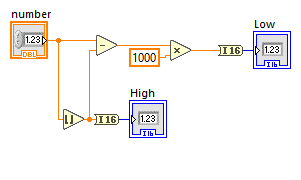
\includegraphics[width=0.5\linewidth]{vis/SplitDouble.PNG}
    \caption{\textit{SplitDouble.vi} is a helper VI that splits a 64 bit-double into two 16-bit words \textbf{High} and \textbf{Low} for Modbus communication. The double is first rounded down to a integer to get the \textbf{High}-part and then that is subtracted from the original number the remaining \textbf{Low}-part is then multiplied by $1000$ because you can't send decimals on this form. On the receiving side the \textbf{Low}-part is divided by $1000$ again as shown in \figref{fig:Splice}.}
    \label{fig:SplitDouble}
\end{figure}

\begin{figure}[H]
    \centering
    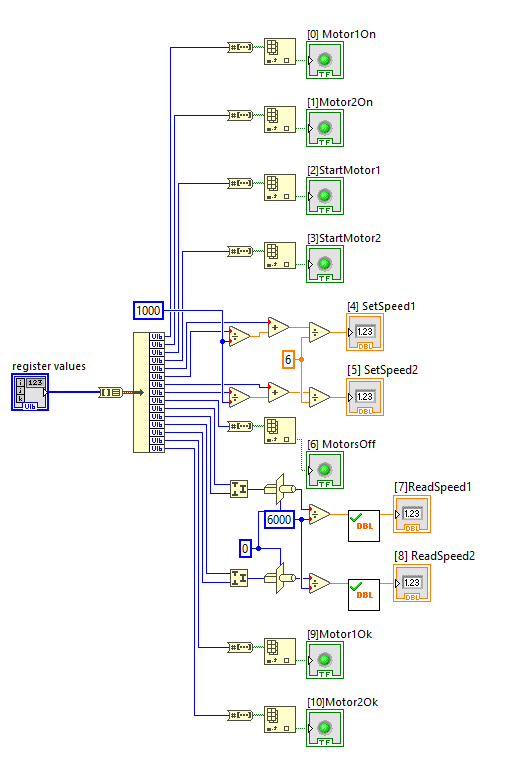
\includegraphics[width=0.5\linewidth]{vis/RegisterSplit.PNG}
    \caption{\textit{RegisterSplit.vi} is a helper VI that splits the register received over modbus to appropriate values for the Labview application.}
    \label{fig:RegisterSplit}
\end{figure}

\subsection{Important VIs}
\begin{figure}[H]
    \centering
    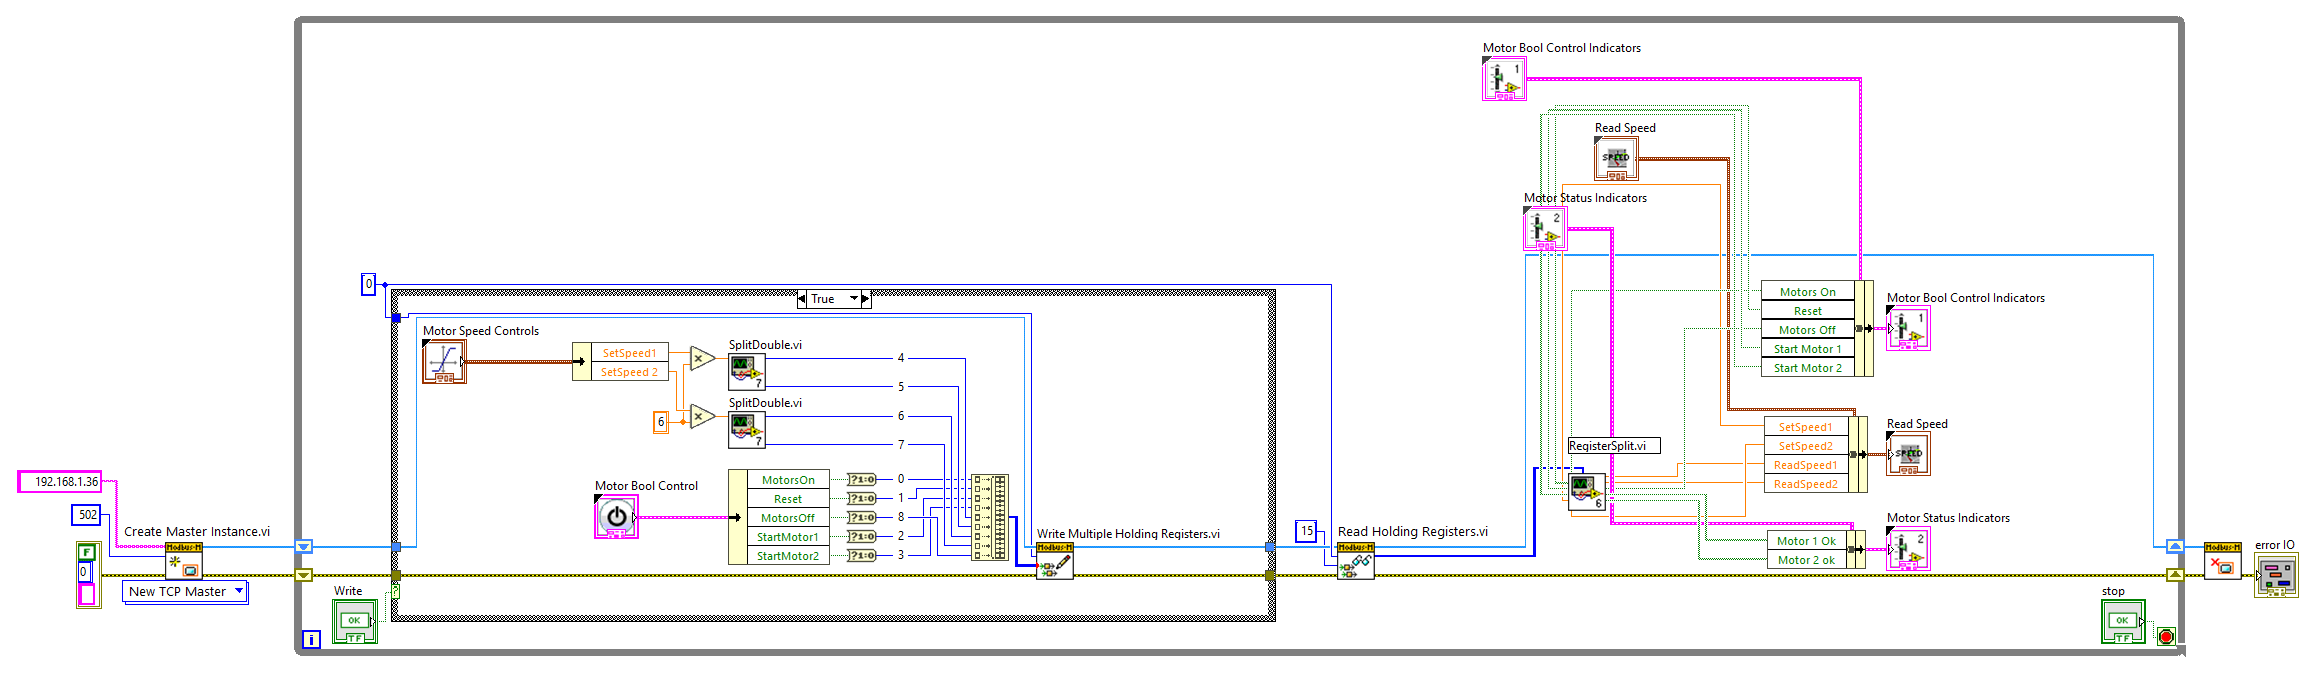
\includegraphics[width=0.75\linewidth]{vis/ModbusIO.PNG}
    \caption{How the modbus connection works on the labview side. This has been adapted to fit better into the \acrshort{mcl}, but functionality is the same.}
    \label{fig:ModbusIO}
\end{figure}

\begin{figure}[H]
    \centering
    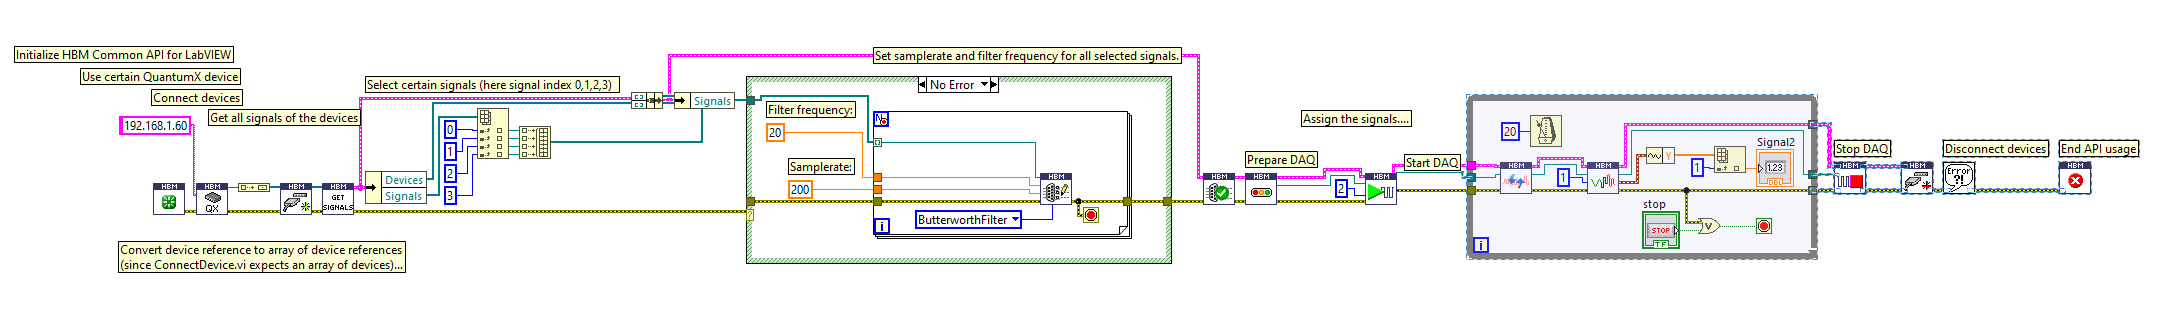
\includegraphics[width=0.75\linewidth]{vis/LoggingSystem.PNG}
    \caption{How the loggin system works. This has been adapted to fit better into the logging loop, but functionality is the same. This example also takes measurements from one channel, the full system utilises all four available channels.}
    \label{fig:Logging}
\end{figure}